\documentclass[../discrete.tex]{subfiles}
\graphicspath{{\subfix{../figures/}}}
\begin{document}
\chapter{Sets, Functions, Sequences, Sums, and Matrices}
\section{Sets}
Sets are used to group objects together. 

A set is an unordered collection of objects, called elements or members of the set. A set contains 
its elements. We write $a \in A$ to denote $a$ is in an element of set $A$. The notation $a\notin A$ 
denotes $a$ is not an element of set $A$.

Here are some sets to remember:
\begin{itemize}
    \item $\mathbb N$ is the set of all natural numbers
    \item $\mathbb Z$ is the set of all integers
    \item $\mathbb Z^+$ is the set of all positive integers
    \item $\mathbb Q$ is the set of all rational numbers
    \item $\mathbb R$ is the set of all real numbers
    \item $\mathbb R^+$ is the set all positive real numbers
    \item $\mathbb C$ is the set of all complex numbers
\end{itemize}

Two sets are equal only if they contain the same elements.

An empty set is notated as \O.

A set with one element is a singleton set.

Set $A$ is a subset of set $B$ and set $B$ is the superset of set $A$ if every element of $A$ is 
also an element of $B$. To indicate $A$ is a subset of $B$ we write $A\subseteq B$. For the equivalent 
superset, we write $B\supseteq A$.

For every nonempty set $S$, there is a guarantee to have at least two subsets, the empty set and the set $S$ itself. 

When we want to say that $A$ is a subset of $B$, but $A\neq B$, we can write $A\subset B$. 

If there are $n$ distinct elements in a set $S$, then the set is finite and $n$ is the cardinality of $S$. 
The cardinality of $S$ is denoted as $|S|$.

Otherwise, the set is infinite if it is not finite.

\begin{definition}
    Given a set $S$, the power set of $S$ is the set of all subsets of the set $S$. The power set of $S$ is defined as $\mathcal{P}(S)$.
\end{definition}

The power set of a set has $2^n$ elements. Because sets are unordered, we need to represent ordered collections using ordered $n$-tuples.
\begin{definition}
    The ordered $n$-tuple $(a_1, a_2,\cdots,a_n)$ is the ordered collection that has $a_1$ as its first element, 
\end{definition}

\section{Set Operations}
If we let $A$ and $B$ be sets, the union of the sets, $A\cup B$, is the set that contains those 
elements that are either in $A$ or $B$, or in both.

The intersection of the sets, $A\cap B$, is the set containing those elements in both $A$ and $B$.

Two sets are called disjoint if the intersection of the sets is an empty set.

The difference of sets $A$ and $B$, or $A-B$ is the set containing those elements that are in $A$ but not in $B$. 
It is also called the complement of $B$ with respect to $A$.

\begin{definition}
    Let $U$ be the universal set. The complement of set $A$ denoted as $\overline{A}$ is the 
    complement of $A$ with respect to $U$. Therefore the complement of the set $A$ is $U-A$.
\end{definition}

Much like the last chapter, there are some set identities and properties
\begin{center}
    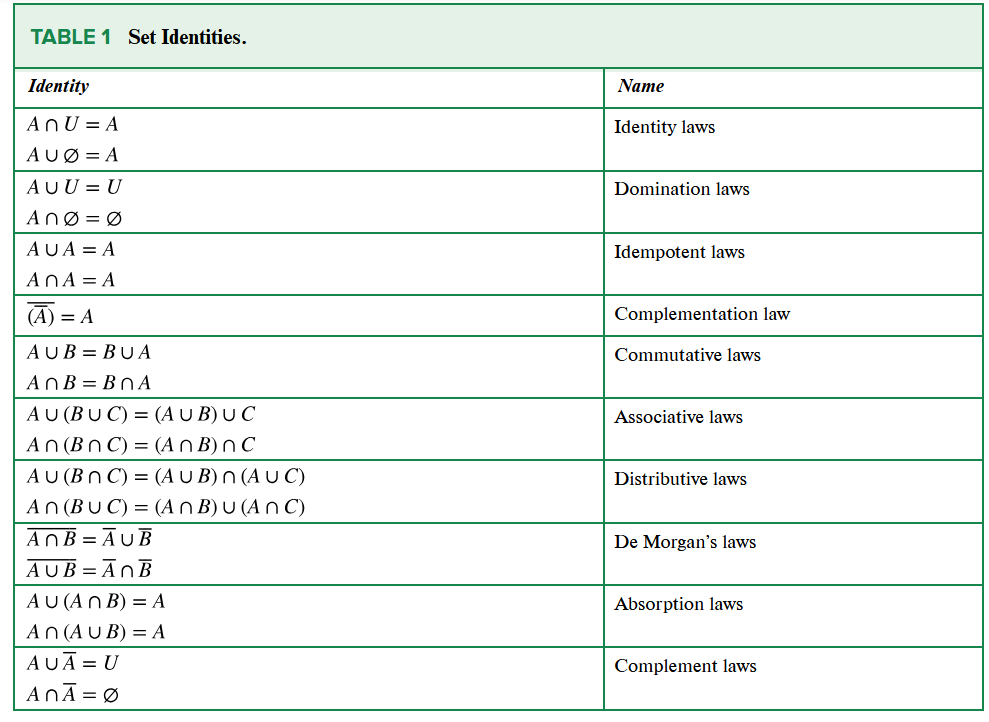
\includegraphics[width=1\textwidth]{discrete2.2.PNG}
\end{center}
Credits to Rosen again.

The union of a collection of sets is the set that contains those elements that are members of at least one set in the collection.

The intersection of a collection of sets is the set that contains those elements that are members of all sets in the collection.

\section{Functions}
\begin{definition}
    Let $A$ and $B$ be empty sets. A function $f$ from $A$ to $B$ is an assignment of exactly 
    one element of $B$ to each element of $A$. We write $f(a)=b$ if $b$ is the unique element of $B$ 
    assigned by the function $f$ to the element $a$ of $A$. If $f$ is a function from $A$ to $B$, 
    we write $f: A\rightarrow B$.
\end{definition}

If $f$ is a function from $A$ to $B$, we say $A$ is the domain of $f$ and $B$ is the codomain of $f$. 
Also if $f(a)=b$, we can say $b$ is the image of $a$ and $a$ is a preimage of $b$. The range, or image, 
is the set of all images of elements of $A$. Also, if $f$ is a function from $A$ to $B$, we say that $f$ 
maps from $A$ to $B$.

A function is called real-valued if its codomain is the set of real numbers and integer-valued if the codomain is the set of integers. 

Some functions never assign the same value to two different domain elements. These are called one-to-one functions, or injective functions.

A function is called surjective or onto when the range and codomain are equal.

If a function is both surjective and injective, then it is bijective.

Only a one-to-one function can be invertible because the inverse of a one-to-one function exists.

\section{Sequences and Summations}
Sequences are ordered lists of elements. The terms of a sequence can be specified by providing a formula for each term of the sequence. 

A sequence is used to represent an ordered list. We use the notation $a_n$ to denote the image of 
the integer $n$. We call $a_n$ a term of the sequence.

A geometric progression is a sequence in the following form:
\[a,ar,ar^2,\cdots,ar^n,\cdots\] 
where the initian term $a$ and common ratio $r$ are real numbers. 

An arithmetic progression is a seuqnece in the form:
\[a,a+d,a+2d,\cdots,a+nd,\cdots\]
where the initial term $a$ and the common difference $d$ are real numbers.

A recurrence relation for the sequence ${a_n}$ is an equation that expresses $a_n$ in 
terms of one or more of the previous terms in the sequence.

A sequence is called a solution of a recurrence relation if its terms satisfy the recurrence relation.

\begin{definition}
    The Fibonacci sequence, $f_0,f_1,f_2,\cdots,$ is defined by the initial conditions 
    $f_0=0, f_1=1,$ and the recurrence relation:
    \[f_n=f_{n-1}+f_{n-2}\]
    for $n=2,3,4,\cdots$.
\end{definition}

Now we introduce the summation notation.

We use the notation $\sum^n_{j=m}a_j$ to represent $a_m+a_{m+1}+\cdots+a_n$.

Here $j$ is the index of summation and is abitrary. 

Sums of terms of geometric progressions commonly arise.

\[\sum^n_{j=0}ar^j=\frac{ar^{n+1}-a}{r-1}\]
when $r\neq 1$ and $(n+1)a$ when $r=1$. 

Here is some formulae for commonly occurring sums:
\begin{center}
    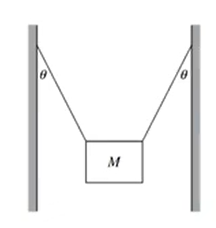
\includegraphics[width=0.5\textwidth]{2.4.PNG}
\end{center}
Credits to Rosen again.
\end{document}